% !TeX root = er.tex

\chapter{Localization}\label{ch.local}

\abstract*{A robot must perform localization, that is, it must know its own position in the environment. It can compute its position relative to landmarks whose position is known using the techniques of classical land surveying. Accurate localization can be achieved using the satellite-based global positioning system (GPS). Probabilistic localization is used in environments where GPS cannot be used, for example, inside a building. Given a map of the environment the robot computes its most likely location based upon data from its sensors. The probabilistic computations can handle uncertainty in the sensors and in the motion of the robot.}

Navigation by odometry (Sect.~\ref{s.odometry}) is prone to errors and can only give an estimate of the real pose of the robot. Moreover, the further the robot moves, the larger the error in the estimation of the pose, especially in the heading. Odometry in a robot can be compared to walking with closed eyes, counting steps until we reach our destination. As with odometry, the further we walk, the more uncertain we are about our location. Even when counting steps, we should open our eyes from time to time to reduce the uncertainty of our location. For a robot, what does it mean to ``count steps'' and ``open our eyes from time to time''? It means that for moving short distances odometry is good enough, but when moving longer distances the robot must determine its position relative to an external reference called a landmark. This process is called \emph{localization}.

Section~\ref{s.landmarks} starts with an activity that you can use to familiarize yourself with the relation between odometry and localization. Section~\ref{s.known-points} presents classical trigonometric techniques used by surveyors to determine the position of a location on earth by measuring angles and distances to positions whose location is known. Section~\ref{s.gps} briefly surveys global positioning systems (GPS) which are now widely used for localization. There are environments where GPS is not effective: in buildings and when very precise positions are needed. Robots in these environments use probabilistic localization techniques that are described in Sects.~\ref{s.prob-local}--\ref{s.uncertain-motion}.

\section{Landmarks}\label{s.landmarks}
\index{landmarks}

Landmarks, such as lines on the ground or doors in a corridor can be detected and identified by the robot and used for localization. The following activity---which uses neither a computer nor a robot---will help you understand the importance of identifying landmarks to correct errors in odometry.

\begin{framed}
\act{Play the landmark game}{landmark-game}
\begin{itemize}
\item Choose a path in your home that requires you to pass several doors, for example, from the bed in your room through a hallway to a sofa in the living room and then back.
\item Close your eyes and walk along the path applying the following rules:
\begin{itemize}
\item You get $30$ points at the beginning of the activity.
\item From time to time you can open your eyes for one second; this action costs $1$ point.
\item If you touch a wall it costs $10$ points.
\end{itemize}
\item How many points do you have when you complete the path?
\item Is it better to open the eyes frequently or to walk the path without ever opening your eyes?
\end{itemize}
\end{framed}

\section{Determining position from objects whose position is known}\label{s.known-points}

In this section we describe two methods which a robot can use to determine its position by measuring angles and distances to an object whose position is known. The first method assumes that the robot can measure the distance to the object and its \emph{azimuth}, the angle of the object relative to north. The second method measures the angles to the object from two different positions. Both methods use trigonometry to compute the coordinates of the robot relative to the object. If the absolute coordinates $(x_0,y_0)$ of the object are known, the absolute coordinates of the robot can then be easily computed.

\subsection{Determining position from an angle and a distance}
\index{localization!angle and distance}

Figure~\ref{fig.angle-distance} shows the geometry of a robot relative to an object. In the diagram the object is denoted by the large dot placed at the origin $(x_0,y_0)$ of a coordinate system. The azimuth of the robot $\theta$ is the angle between north and the forward direction of the robot; it can be measured by a compass. A laser scanner is used to measure the distance $s$ to the object and the angle $\phi$ between the forward direction of the robot and the object. The relative coordinates $\Delta x$ and $\Delta y$ can be determined by simple trigonometry:
\[
\Delta x = s \sin (\theta-\phi), \;\;\; \Delta y = s \cos (\theta-\phi)\,.
\]
From the known absolute coordinates of the object $(x_0,y_0)$, the coordinates of the robot can be determined.

\begin{figure}
\begin{center}
\begin{tikzpicture}[scale=1.2]
\draw (-1,3) -- node[above] { $\Delta x$ } +(7,0);
\pic[rotate=15,scale=.8] at (0,0) { robot };
\draw[dashed] (0,0) -- +(15:6cm);
\draw[dashed] (0,0) -- +(30:7cm);
\draw (0,0) -- node[left] { $\Delta y$ } +(90:4cm);
\draw (5.2,0) -- +(0,4);
\draw[fill] (5.2,3) circle [radius=2pt];
\draw[red,thick] (0,2.3cm) arc[radius=2.3cm, start angle=90, delta angle = -75];
\draw[blue,thick] (30:3.1cm)  arc[radius=3.1cm, start angle=30, delta angle = -15];
\draw[thick] (90:1.5cm) arc[radius=1.5cm, start angle=90, delta angle = -60];
\node at (5.7,2.8) { $(x_0,y_0)$ };
\node at (60:2.6cm) { $\theta$ };
\node at (60:1.8cm) { $\theta-\phi$ };
\node at (22.5:3.3) { $\phi$ };
\end{tikzpicture}
\caption{Determining position from an angle and a distance}\label{fig.angle-distance}
\end{center}
\end{figure}

\begin{framed}
\act{Determining position from an angle and a distance}{position-distance-angle}
\begin{itemize}
\item Implement the algorithm.
\item To measure the azimuth place the robot lined up with a edge of the table and call it north. Measure the angle to the object using several horizontal sensors or using one sensor and rotating either the sensor or the robot.
\item The distance and the angle are measured from the position where the sensor is mounted, which is not necessarily the center of the robot. You may have to make corrections for this.
\end{itemize}
\end{framed}

\subsection{Determining position by triangulation}
\index{localization!triangulation}
\index{triangulation}

\emph{Triangulation} is used for determining coordinates when it is difficult or impossible to measure distances. It was widely used in surveying before lasers were available, because it was impossible to measure long distances accurately. The principle of triangulation is that from two angles of a triangle and the length of the included side, you can compute the lengths of the other sides. Once these are known, the relative position of a distant object can be computed.

Figure~\ref{fig.triangulation} shows the robot measuring the angles $\alpha$ and $\beta$ to the object from two positions separated by a distance $c$. If the two positions are close, the distance can be measured using a tape measure. Alternatively, the distance can be measured by odometry as the robot moves from one position to another, though this may be less accurate. In surveying, if the coordinates of the two positions are known, the distance between them can be computed and used to determine the coordinates of the object.

The lengths $a$ and $b$ are computed using the \emph{law of sines}:
\begin{displaymath}
\frac{a}{\sin\alpha'} = \frac{b}{\sin\beta'} = \frac{c}{\sin\gamma}\,,
\end{displaymath}
where $\alpha' = 90^{\circ} - \alpha, \: \beta' = 90^{\circ} - \beta$ are the interior angles of the triangle. To use the law, we need $c$, which has been measured, and $\gamma$, which is:
\begin{displaymath}
\gamma = 180^{\circ}-\alpha'-\beta' = 180^{\circ} - (90^{\circ} -
\alpha) - (90^{\circ} - \beta) = \alpha + \beta\,.
\end{displaymath}
From the law of sines:
\begin{displaymath}
b = \frac{c\sin\beta'}{\sin\gamma} =
\frac{c\sin (90^{\circ} - \beta)}{\sin (\alpha + \beta)} =
\frac{c\cos\beta}{\sin (\alpha + \beta)}\,.
\end{displaymath}
A similar computation gives $a$.

\begin{figure}
\begin{center}
\begin{tikzpicture}
\coordinate (top) at (0,2);
\coordinate (bottom) at (0,-2);
\coordinate (object) at (5,0);
\pic[scale=.8] at (top) { robot };
\pic[scale=.8] at (bottom) { robot };
\draw[fill] (object) circle [radius=3pt] node[xshift=-15pt] { $\gamma$ };
\draw (top) -- +(5,0);
\draw (bottom) -- +(5,0);
\draw (top) -- node[above] { $a$ } (object);
\draw (bottom) -- node[below] { $b$ } (object);
\draw (top) -- node[left] { $c$ } (bottom);
\node[xshift=42pt,yshift=-8pt] at (top) { $\beta$ };
\node[xshift=15pt,yshift=-25pt] at (top) { $\beta'$ };
\node[xshift=42pt,yshift=8pt] at (bottom) { $\alpha$ };
\node[xshift=15pt,yshift=25pt] at (bottom) { $\alpha'$ };
\end{tikzpicture}
\caption{Triangulation}\label{fig.triangulation}
\end{center}
\end{figure}


\begin{framed}
\act{Determining position by triangulation}{triangulation}
\begin{itemize}
\item Implement triangulation.
\item Initially, perform a measurement of the angle at one position and then pick the robot up and move it to a new position for the second measurement, carefully measuring the distance $c$.
\item Alternatively, cause the robot move by itself from the first position to the second, calculating $c$ by odometry.
\end{itemize}
\end{framed}

\section{Global positioning system}\label{s.gps}
\index{global positioning system}

In recent years, the determination of location has been made easier and more accurate with the introduction of the \emph{Global Positioning System (GPS)}.\footnote{The generic term is \emph{global navigation satellite system (GNSS)} since GPS refers to the specific system operated by the United States. Similar systems are operated by the European Union (Galileo), Russia (GLONASS) and China (BeiDou), but GPS is frequently used to refer to all such systems and we do so here.} GPS navigation is based upon orbiting satellites. Each satellite knows its precise position in space and its local time. The position is sent to the satellite by ground stations and the time is measured by a highly accurate atomic clock on the satellite.

A GPS receiver must be able to receive data from four satellites. For this reason, a large number of satellites ($24$--$32$) is needed so that there is always a line-of-sight between any location and at least four satellites. From the time signals sent by a satellite, the distances from the satellites to the receiver can be computed by multiplying the times of travel by the speed of light. These distances and the known locations of the satellites enable the computation of the three-dimensional position of the receiver: latitude, longitude and elevation.

The advantage of GPS navigation is that it is accurate and available anywhere with no additional equipment beyond an electronic component that is so small and inexpensive that it is found in every smartphone. There are two problems with GPS navigation:
\begin{itemize}
\item The position error is roughly $10$ meters. While this is sufficient to navigate your car to choose the correct the road at an intersection, it is not sufficient to perform tasks that need higher accuracy, for example, parking your car.
\item GPS signals are not strong enough for indoor navigation and are subject to interference in dense urban environments.
\end{itemize}

\begin{quote}
\begin{center}
\textbf{Relativity and GPS}
\end{center}
You have certainly heard of Albert Einstein's theory of relativity and probably considered it to be an esoteric theory of interest only to physicists. However, Einstein's theories are used in the GPS computations! According to the special theory of relativity, the clocks on the satellites run \emph{slower} than they do on the Earth (by 7.2 microseconds per day), because the satellites are moving fast relative to the Earth. According to the general theory of relativity, the clocks run \emph{faster} (by 45.9 microseconds per day), because the force of the Earth's gravity is smaller at the distant satellite than it is for us on the surface. The two effects do not cancel out and a correction factor is used when broadcasting the time signals.
\end{quote}

\section{Probabilistic localization}\label{s.prob-local}
\index{localization!probabilistic}

Consider a robot that is navigating within a known environment for which it has a \emph{map}. The following map shows a wall with five doors (dark gray) and three areas where there is no door (light gray):

\begin{center}
% Robot trying to localize 1
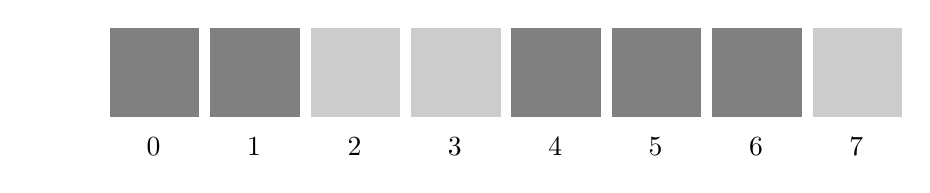
\begin{tikzpicture}[scale=.75]
\path (-1.4cm,0) -- (0,0);  % Space for robot
\foreach \n/\x/\color in
  {0/0/100, 1/1.7/100, 2/3.4/40, 3/5.1/40,
   4/6.8/100, 5/8.5/100, 6/10.2/100, 7/11.9/40} {
    \draw[fill,color=gray!\color] (\x,0) rectangle +(1.5,1.5);
    \node[xshift=.55cm] at (\x, -5mm) {\p{\n}};
}
\end{tikzpicture}
\end{center}

For clarity the doors and walls are drawn as if they are on the floor and the robot moves over them, measuring intensity with ground sensors.

The task of the robot is to enter a specific door, say the one at position 4. But how can the robot know where it is? By odometry, the robot can determine its current position given a known starting position. For example, if the robot is at the left end of the wall:
\begin{center}
% Robot trying to localize 2
\begin{tikzpicture}[scale=.75]
\path (-1.4cm,0) -- (0,0);  % Space for robot
\foreach \n/\x/\color in
  {0/0/100, 1/1.7/100, 2/3.4/40, 3/5.1/40,
   4/6.8/100, 5/8.5/100, 6/10.2/100, 7/11.9/40} {
    \draw[fill,color=gray!\color] (\x,0) rectangle +(1.5,1.5);
    \node[xshift=.55cm] at (\x, -5mm) {\p{\n}};
}
\pic[scale=.5,fill] at (-1.1cm,7.5mm) { robot };
\end{tikzpicture}
\end{center}
it knows that it has to move five times the width of each door, while if the robot is at the following position:
\begin{center}
% Robot trying to localize 3
\begin{tikzpicture}[scale=.75]
\path (-1.4cm,0) -- (0,0);  % Space for robot
\foreach \n/\x/\color in
  {0/0/100, 1/1.7/100, 2/3.4/40, 3/5.1/40,
   4/6.8/100, 5/8.5/100, 6/10.2/100, 7/11.9/40} {
    \draw[fill,color=gray!\color] (\x,0) rectangle +(1.5,1.5);
    \node[xshift=.55cm] at (\x, -5mm) {\p{\n}};
}
\pic[scale=.5,fill] at (5.5cm,7.5mm) { robot };
\end{tikzpicture}
\end{center}
the required door is the next one to the right. Because of errors in odometry, it is quite likely that as time goes by the robot will get lost. In this section, we implement a one-dimensional version of a probabilistic \emph{Markov localization algorithm}\index{Markov algorithm} that takes into account uncertainty in the sensors and in the robot's motion, and returns the most probable locations of the robot.

Appendix~\ref{a.bayes} contains a short tutorial on conditional probability and Bayes rule, including an example of the details of the calculations of uncertainty.

\subsection{Sensing increases certainty}

Consider a robot in the above environment of walls and doors that has no information as to its location. The robot assigns a probability to the eight positions where it might be located. Initially, it has no idea where it is, so each position will be assigned the probability $b[i]=1.0/8=.125\approx .13$, where $b$ is called the \emph{belief array}:\footnote{All probabilities will be rounded to two decimal digits for display.}
\begin{center}
\begin{tikzpicture}
\draw (0,3) node[left] {\p{1.0}} -- node[left] {$p$} (0,0) node[left] {\p{0.0}} -- node[below,yshift=-4mm] {$b$} (8,0);
\foreach \n/\v in {0/.13, 1/.13, 2/.13, 3/.13, 4/.13, 5/.13, 6/.13, 7/.13}
  \pic { bar=\n/\v };
\foreach \n in {.5, 1.5, 4.5, 5.5, 6.5}
  \node at (\n,3) {$\bullet$};
\pic[scale=.2] at (4.4,2.5) { robot };
\end{tikzpicture}
\end{center}
\vspace{-1ex}
In the plots the dots denote the positions of the doors and a small icon indicates the actual position of the robot which is facing right.

Suppose now that the robot's sensors detect a dark gray area. Its uncertainty is reduced, because it knows that it must be in front of one of the five doors. The belief array shows $.2$ for each of the doors and $.0$ for each of the walls:
\begin{center}
\begin{tikzpicture}
\draw (0,3) node[left] {\p{1.0}} -- node[left] {$p$} (0,0) node[left] {\p{0.0}} -- node[below,yshift=-4mm] {$b$} (8,0);
\foreach \n/\v in {0/.2, 1/.2, 2/.0, 3/.0, 4/.2, 5/.2, 6/.2, 7/.0}
  \pic { bar=\n/\v };
\foreach \n in {.5, 1.5, 4.5, 5.5, 6.5}
  \node at (\n,3) {$\bullet$};
\pic[scale=.2] at (4.4,2.5) { robot };
\end{tikzpicture}
\end{center}
\vspace{-1ex}
Next the robot moves forwards and again senses a dark gray area. There are now only three possibilities: it was at position 0 and moved to 1, it was at 4 and moved to 5, or it was at 5 and moved to 6. If the robot's initial position were 1 or 6, after moving right it would no longer detect a dark gray area, so it could not have been there. The probability is now $.33$ for each of the three positions 1, 4, 5:
\begin{center}
\begin{tikzpicture}
\draw (0,3) node[left] {\p{1.0}} -- node[left] {$p$} (0,0) node[left] {\p{0.0}} -- node[below,yshift=-4mm] {$b$} (8,0);
\foreach \n/\v in {0/.0, 1/.33, 2/.0, 3/.0, 4/.0, 5/.33, 6/.33, 7/.0}
  \pic { bar=\n/\v };
\foreach \n in {.5, 1.5, 4.5, 5.5, 6.5}
  \node at (\n,3) {$\bullet$};
\pic[scale=.2] at (5.4,2.5) { robot };
\end{tikzpicture}
\end{center}
\vspace{-1ex}
After the next step of the robot, if it again detects a door, it is without doubt at position 6:
\begin{center}
\begin{tikzpicture}
\draw (0,3) node[left] {\p{1.0}} -- node[left] {$p$} (0,0) node[left] {\p{0.0}} -- node[below,yshift=-4mm] {$b$} (8,0);
\foreach \n/\v in {0/.0, 1/.0, 2/.0, 3/.0, 4/.0, 5/.0, 6/1.0, 7/.0}
  \pic { bar=\n/\v };
\foreach \n in {.5, 1.5, 4.5, 5.5, 6.5}
  \node at (\n,3) {$\bullet$};
\pic[scale=.2] at (6.4,2.5) { robot };
\end{tikzpicture}
\end{center}
\vspace{-1ex}
\noindent{}If the robot did not detect a door, it is either at position 2 or position 7:
\begin{center}
\begin{tikzpicture}
\draw (0,3) node[left] {\p{1.0}} -- node[left] {$p$} (0,0) node[left] {\p{0.0}} -- node[below,yshift=-4mm] {$b$} (8,0);
\foreach \n/\v in {0/.0, 1/.0, 2/.5, 3/.0, 4/.0, 5/.0, 6/.0, 7/.5}
  \pic { bar=\n/\v };
\foreach \n in {.5, 1.5, 4.5, 5.5, 6.5}
  \node at (\n,3) {$\bullet$};
\end{tikzpicture}
\end{center}
\vspace{-1ex}
The robot maintains a belief array and integrates new data when it detects the presence or absence of a door. As time goes on, the uncertainty decreases: the robot  knows with greater certainty where it is actually located. In this example, eventually the robot knows its position in front of door $6$ with complete certainty or it has reduced its uncertainty to one of the two positions $2,7$.

\subsection{Uncertainty in sensing}

The values returned by the robot's sensors reflect the intensity of the light reflected by the gray colors of the doors and walls. If the difference in the color of a dark gray door and a light gray wall is not very great, the robot may occasionally detect a dark gray door as a light gray wall, or conversely. This can occur due to changes in the ambient lighting or to errors in the sensors themselves. It follows that the robot cannot distinguish between the two with complete certainty.

We model this aspect of the world by assigning probabilities to the detection. If the robot senses dark gray, we specify that the probability is $.9$ that it has correctly detected a door and $.1$ that it has mistakenly detected a wall where there was in fact a door. Conversely, if it senses light gray, the probability is $.9$ that it has correctly detected a wall and $.1$ that it has mistakenly detected a door where there was a wall.

We continue to display the computations in graphs but you may find it easier to follow them in Table~\ref{tab.uncertain-sensing}. Each row represents the belief array of the robot following the action written in the first column.

\begin{table}
\caption[Localization with uncertainty in sensing]{Localization with uncertainty in sensing\newline{}sensor=after multiplying by the sensor uncertainty\newline{}norm=after normalization\newline{}right=after moving right one position}\label{tab.uncertain-sensing}
\setlength{\tabcolsep}{6pt}
\begin{tabular}{l|rrrrrrrr}
\svhline\noalign{\smallskip}
position&\multicolumn{1}{c}{$0$}&\multicolumn{1}{c}{$1$}&\multicolumn{1}{c}{$2$}&\multicolumn{1}{c}{$3$}&\multicolumn{1}{c}{$4$}&\multicolumn{1}{c}{$5$}&\multicolumn{1}{c}{$6$}&\multicolumn{1}{c}{$7$}\\
door?&\multicolumn{1}{c}{$\bullet$}&\multicolumn{1}{c}{$\bullet$}&&&\multicolumn{1}{c}{$\bullet$}&\multicolumn{1}{c}{$\bullet$}&\multicolumn{1}{c}{$\bullet$}&\\
\svhline\noalign{\smallskip}
initial &$0.13$ & $0.13$ & $0.13$ & $0.13$ & $0.13$ & $0.13$ & $0.13$ & $0.13$\\
sensor  &$0.11$ & $0.11$ & $0.01$ & $0.01$ & $0.11$ & $0.11$ & $0.11$ & $0.01$\\
norm    &$0.19$ & $0.19$ & $0.02$ & $0.02$ & $0.19$ & $0.19$ & $0.19$ & $0.02$\\
\hline
right   &$0.02$ & $0.19$ & $0.19$ & $0.02$ & $0.02$ & $0.19$ & $0.19$ & $0.19$\\
sensor  &$0.02$ & $0.17$ & $0.02$ & $0.00$ & $0.02$ & $0.17$ & $0.17$ & $0.02$\\
norm    &$0.03$ & $0.29$ & $0.03$ & $0.00$ & $0.03$ & $0.29$ & $0.29$ & $0.03$\\
\hline
right   &$0.03$ & $0.03$ & $0.29$ & $0.03$ & $0.00$ & $0.03$ & $0.29$ & $0.29$\\
sensor  &$0.03$ & $0.03$ & $0.03$ & $0.00$ & $0.00$ & $0.03$ & $0.26$ & $0.03$\\
norm    &$0.07$ & $0.07$ & $0.07$ & $0.01$ & $0.01$ & $0.07$ & $0.63$ & $0.07$\\
\noalign{\smallskip}\svhline\noalign{\smallskip}
\end{tabular}
\end{table}

Initially, after sensing dark gray at a position where there is a door, we only know with probability $.125\times 0.9 = .1125$ that a door has been correctly detected; however, there is still a $.125\times .1= .0125$ probability that it has mistakenly detected a wall. After normalizing (Appendix~\ref{a.normalize}), the belief array is:
\begin{center}
\begin{tikzpicture}
\draw (0,3) node[left] {\p{1.0}} -- node[left] {$p$} (0,0) node[left] {\p{0.0}} -- node[below,yshift=-4mm] {$b$} (8,0);
\foreach \n/\v in {0/.19, 1/.19, 2/.02, 3/.02, 4/.19, 5/.19, 6/.19, 7/.02}
  \pic { bar=\n/\v };
\foreach \n in {.5, 1.5, 4.5, 5.5, 6.5}
  \node at (\n,3) {$\bullet$};
\pic[scale=.2] at (4.4,2.5) { robot };
\end{tikzpicture}
\end{center}
\vspace{-1ex}
What happens when the robot moves one position to the right? Its belief array must also move one position to the right. For example, the probability $.19$ that the robot was at position $1$ now becomes the probability that it is at position $2$. Similarly, the probability $.02$ that the robot was at position $3$ now becomes the probability that it is at position $4$. The probability is now $0$ that the robot is at position $0$ and the probability $b_7$ becomes $b_8$, so the indices become $1$--$8$ instead of $0$--$7$. To simplify the computations and the diagrams in the example, the indices $0$--$7$ are retained and the value of $b_8$ is stored in $b_0$ as if the map were cyclic. The belief array after the robot moves right is:
\begin{center}
\begin{tikzpicture}
\draw (0,3) node[left] {\p{1.0}} -- node[left] {$p$} (0,0) node[left] {\p{0.0}} -- node[below,yshift=-4mm] {$b$} (8,0);
\foreach \n/\v in {0/.02, 1/.19, 2/.19, 3/.02, 4/.02, 5/.19, 6/.19, 7/.19}
  \pic { bar=\n/\v };
\foreach \n in {.5, 1.5, 4.5, 5.5, 6.5}
  \node at (\n,3) {$\bullet$};
\pic[scale=.2] at (5.4,2.5) { robot };
\end{tikzpicture}
\end{center}
\vspace{-1ex}
If the robot again senses dark gray, the probability of being at positions 1, 5 or 6 should increase. Computing the probabilities and normalizing gives:
\begin{center}
\begin{tikzpicture}
\draw (0,3) node[left] {\p{1.0}} -- node[left] {$p$} (0,0) node[left] {\p{0.0}} -- node[below,yshift=-4mm] {$b$} (8,0);
\foreach \n/\v in {0/.03, 1/.29, 2/.03, 3/.0, 4/.03, 5/.29, 6/.29, 7/.03}
  \pic { bar=\n/\v };
\foreach \n in {.5, 1.5, 4.5, 5.5, 6.5}
  \node at (\n,3) {$\bullet$};
\pic[scale=.2] at (5.4,2.5) { robot };
\end{tikzpicture}
\end{center}
\vspace{-1ex}
Now the robot moves right again:
\begin{center}
\begin{tikzpicture}
\draw (0,3) node[left] {\p{1.0}} -- node[left] {$p$} (0,0) node[left] {\p{0.0}} -- node[below,yshift=-4mm] {$b$} (8,0);
\foreach \n/\v in {0/.03, 1/.03, 2/.29, 3/.03, 4/.0, 5/.03, 6/.29, 7/.29}
  \pic { bar=\n/\v };
\foreach \n in {.5, 1.5, 4.5, 5.5, 6.5}
  \node at (\n,3) {$\bullet$};
\pic[scale=.2] at (6.4,2.5) { robot };
\end{tikzpicture}
\end{center}
\vspace{-1ex}
\noindent{}and senses a third dark gray area. The belief array becomes:
\begin{center}
\begin{tikzpicture}
\draw (0,3) node[left] {\p{1.0}} -- node[left] {$p$} (0,0) node[left] {\p{0.0}} -- node[below,yshift=-4mm] {$b$} (8,0);
\foreach \n/\v in {0/.07, 1/.07, 2/.07, 3/.01, 4/.0, 5/.07, 6/.63, 7/.07}
  \pic { bar=\n/\v };
\foreach \n in {.5, 1.5, 4.5, 5.5, 6.5}
  \node at (\n,3) {$\bullet$};
\pic[scale=.2] at (6.4,2.5) { robot };
\end{tikzpicture}
\end{center}
\vspace{-1ex}
Not surprisingly, the robot is almost certainly at position 6.

\begin{framed}
\act{Localization with uncertainty in the sensors}{local-uncertain}
\begin{itemize}
\item Implement probabilistic localization with uncertainty in the sensor.
\item How does the behavior of the algorithm change when the uncertainty is changed?
\item Run the algorithm for different starting positions of the robot.
\end{itemize}
\end{framed}

\section{Uncertainty in motion}\label{s.uncertain-motion}

As well as uncertainty in the sensors, robots are subject to uncertainty in their motion. We can ask the robot to move one position to the right, but it might move two positions, or it might move very little and remain in its current position. Let us modify the algorithm to take this uncertainty into account.

Let $b$ be the belief array. The belief array is updated using the formula:\begin{displaymath}
b'_i = p_i \, b_i\,,
\end{displaymath}
where $b'_i$ is the new value of $b_i$ and $p_i$ is the probability of detecting a door (in the example, $p_i$ is $0.9$ for $i=0,1,4,5,6$ and $p_i$ is $0.1$ for $i=2,3,7$). If the motion is certain the robot moves one position to the right, but with uncertain motion, the following computation takes into account the probabilities $q_j$ that the robot actually moves $j=0,1,2$ positions:
\begin{displaymath}
b'_i = p_i \,(b_{i-2}\, q_2 + b_{i-1}\, q_1 + b_{i}\, q_0)\,,
\end{displaymath}
as shown in the following diagram:
\begin{center}
\begin{tikzpicture}[scale=1.1]
\begin{scope}[every node/.style={draw,rectangle,minimum size=1cm}]
\node (b2)  {$b_{i-2}$};
\node (b1)  [right=of b2] {$b_{i-1}$};
\node (b)   [right=of b1] {$b_{i}$};
\node (b2p) [below=of b2] {};
\node (b1p) [below=of b1] {};
\node (bp)  [below=of b]  {$b'$};
\end{scope}
\draw[->] (b2.south) -- node[below,near start] {$q_2$} (bp.north west);
\draw[->] (b1.south) -- node[above] {$q_1$} (bp.north);
\draw[->] (b.south)  -- node[above,near end,xshift=6pt] {$q_0$} (bp.north east);
\end{tikzpicture}
\end{center}
It is highly likely that the robot will move correctly, so reasonable values are $q_1=0.8$ and $q_0=q_2=0.1$. With these values for the uncertainty of the motion and the previous values for $p_i$, the calculation of the belief array after three moves is shown in Table~\ref{tab.uncertain-sensing-motion} and its final value is shown in the following diagram:
\begin{center}
\begin{tikzpicture}
\draw (0,3) node[left] {\p{1.0}} -- node[left] {$p$} (0,0) node[left] {\p{0.0}} -- node[below,yshift=-4mm] {$b$} (8,0);
\foreach \n/\v in {0/.11, 1/.21, 2/.05, 3/.01, 4/.02, 5/.13, 6/.43, 7/.05}
  \pic { bar=\n/\v };
\foreach \n in {.5, 1.5, 4.5, 5.5, 6.5}
  \node at (\n,3) {$\bullet$};
\pic[scale=.2] at (1.4,2.5) { robot };
\node at (2,2.5) {\p{?}};
\pic[scale=.2] at (6.4,2.5) { robot };
\node at (7,2.5) {\p{?}};
\end{tikzpicture}
\end{center}
The robot is likely at position 6, but we are less certain because the probability is only $.43$ instead of $.63$. There is a non-negligible probability of $.21$ that the robot is at position 1.

\begin{table}
\caption[Localization with uncertainty in sensing and motion]{Localization with uncertainty in sensing and motion\newline{}sensor=after multiplying by the sensor uncertainty\newline{}norm=after normalization\newline{}right=after moving right one position}\label{tab.uncertain-sensing-motion}
\setlength{\tabcolsep}{6pt}
\begin{tabular}{l|rrrrrrrr}
\svhline\noalign{\smallskip}
position&\multicolumn{1}{c}{$0$}&\multicolumn{1}{c}{$1$}&\multicolumn{1}{c}{$2$}&\multicolumn{1}{c}{$3$}&\multicolumn{1}{c}{$4$}&\multicolumn{1}{c}{$5$}&\multicolumn{1}{c}{$6$}&\multicolumn{1}{c}{$7$}\\
door?&\multicolumn{1}{c}{$\bullet$}&\multicolumn{1}{c}{$\bullet$}&&&\multicolumn{1}{c}{$\bullet$}&\multicolumn{1}{c}{$\bullet$}&\multicolumn{1}{c}{$\bullet$}&\\
\svhline\noalign{\smallskip}
initial  & $0.13$ & $0.13$ & $0.13$ & $0.13$ & $0.13$ & $0.13$ & $0.13$ & $0.13$\\
sensor & $0.11$ & $0.11$ & $0.01$ & $0.01$ & $0.11$ & $0.11$ & $0.11$ & $0.01$\\
norm     & $0.19$ & $0.19$ & $0.02$ & $0.02$ & $0.19$ & $0.19$ & $0.19$ & $0.02$\\
\hline
right    & $0.05$ & $0.17$ & $0.17$ & $0.04$ & $0.04$ & $0.17$ & $0.19$ & $0.17$\\
sensor & $0.05$ & $0.17$ & $0.02$ & $0.00$ & $0.03$ & $0.15$ & $0.17$ & $0.02$\\
norm     & $0.08$ & $0.27$ & $0.03$ & $0.01$ & $0.06$ & $0.25$ & $0.28$ & $0.03$\\
\hline
right    & $0.06$ & $0.09$ & $0.23$ & $0.05$ & $0.01$ & $0.07$ & $0.23$ & $0.25$\\
sensor & $0.05$ & $0.10$ & $0.02$ & $0.01$ & $0.01$ & $0.06$ & $0.21$ & $0.02$\\
norm     & $0.11$ & $0.21$ & $0.05$ & $0.01$ & $0.02$ & $0.13$ & $0.43$ & $0.05$\\
\noalign{\smallskip}\svhline\noalign{\smallskip}
\end{tabular}
\end{table}

\begin{framed}
\act{Localization with uncertainty in the motion}{local-motion}
\begin{itemize}
\item Implement probabilistic localization with uncertainty in the computation of the motor power.
\item How does the behavior of the algorithm change when the uncertainty is changed?
\item Run the algorithm for different starting positions of the robot.
\end{itemize}
\end{framed}


\section{Summary}

Odometry provides an estimation of the position of a robot. A robot can use surveying techniques to compute its position relative to an object of known position. GPS gives excellent data on location, however, it may not be accurate enough and interference with reception from the satellites limits its use in indoor environments. If there are multiple known objects that the robot can sense and if it has a map of its environment, it can use probabilistic localization to estimate its position with high probability, although the probability will be reduced if there is a lot of uncertainty in the sensors or in the motion of the robot.

\section{Further reading}

Probabilistic methods in robotics are treated in depth in \cite{thrun}. There is a wealth of information on GPS at \url{http://www.gps.gov}. An implementation of probabilistic localization using the Thymio educational robot is described in \cite{wang2016dars}.

\bibliographystyle{spmpsci}
\bibliography{er}
